\subsection{Python-Based Model Implementation}

Our study provides a Python-based implementation library for both the formal model and the insight model. The library incorporates the three notions of knowledge wealth discussed in \autoref{wealth-formal-model}, as well as the insight model outlined in \autoref{insight-model}. While the model is platform-agnostic, i.e., it can be applied to any KG, we focus its implementation on Wikidata for demonstrating its use cases. Wikidata is specifically chosen because of the availability of Wikidata Query Service which  facilitates structured queries over its data.

The notions of wealth are implemented at the query level, meaning that the filters and aggregations based on each wealth definition are directly embedded in SPARQL queries. The flow begins with defining class filters to specify the entities of interest. Next, SPARQL querying is performed using Wikidata Query Service to retrieve RDF triples matching the specified criteria and aggregate them according to the selected notion of wealth. The extracted data is then structured into pandas DataFrames, enabling further analysis through the insight model using Python libraries.

In our implementation, we only consider direct properties and exclude blank nodes to reduce complexity and maintain data quality. The complete flow of the formal model and insight model usage is illustrated in \autoref{fig:model-implementation}.

\begin{figure}[!htbp]
    \centering
    % 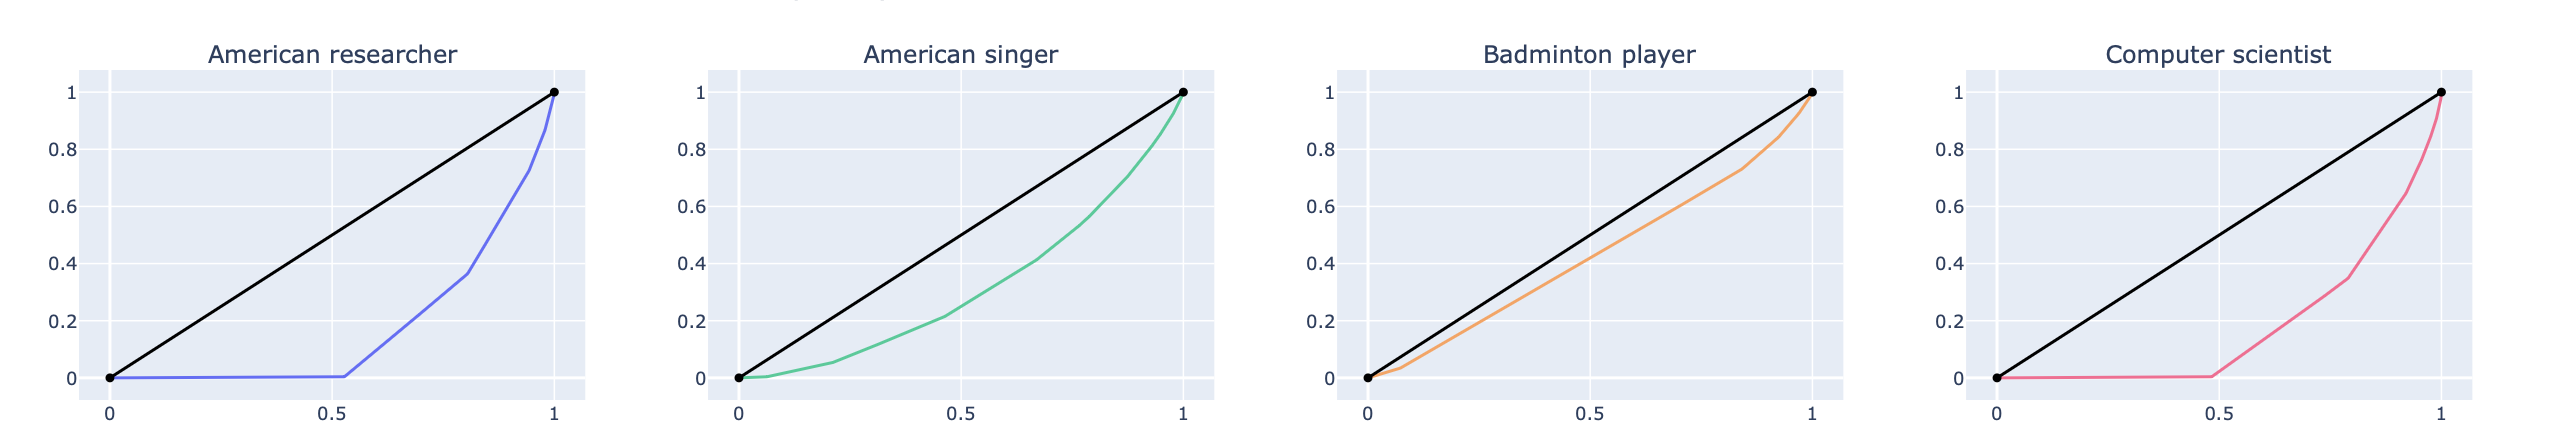
\includegraphics[scale=.5]{Gini - Pure Literal}
    \makebox[\textwidth][c]{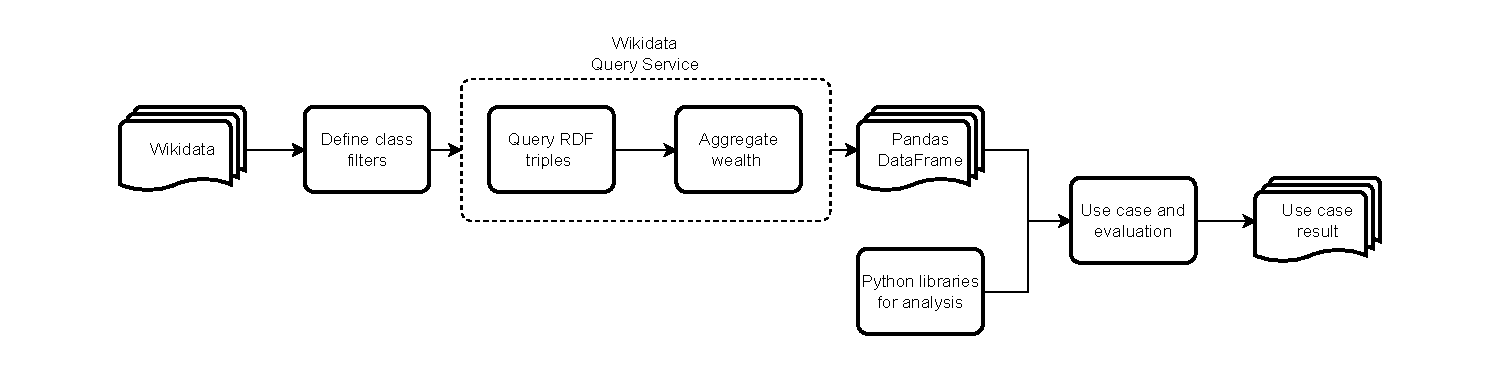
\includegraphics[width=1\textwidth]{Model Implementation.pdf}}%
    \caption{Model implementation and evaluation flow using Python Jupyter Notebook} \label{fig:model-implementation}
\end{figure}